% =========================================================================== %

\begin{frame}[t,plain]
\titlepage
\end{frame}

% =========================================================================== %

\begin{frame}
%
\begin{columns}[T]
\column{.5\linewidth}
\begin{center}
	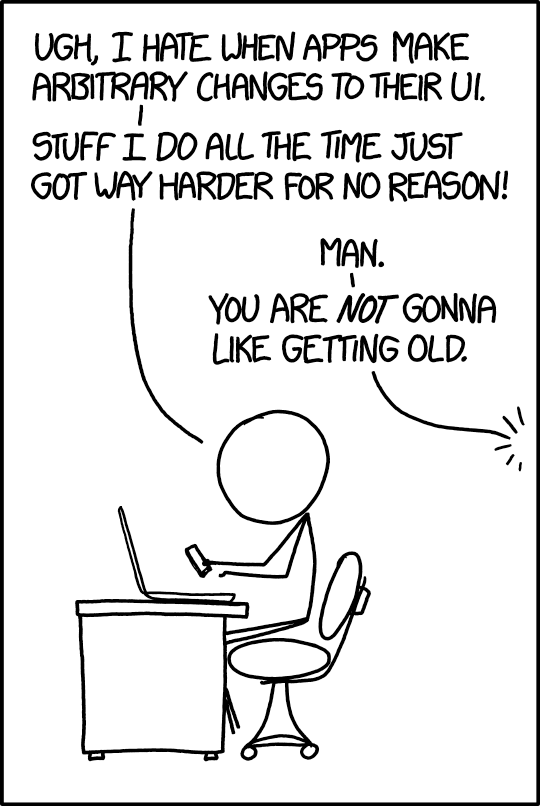
\includegraphics[width=.67\linewidth]{./gfx/12-xkcd-change}
\end{center}
%
\column{.5\linewidth}
\begin{Large}
	{UI Change}
\end{Large}
%
\begin{center}
	\vspace{60pt}
	\emph{I know they said this change is permanent, but surely when they hear how much we're complaining someone will find a way to change things back.}

	\vspace{6pt}
	Source: \url{https://xkcd.com/1770/}
\end{center}
\end{columns}

%
\end{frame}

% =========================================================================== %

\begin{frame}{Scope For Today}
%
\begin{itemize}
\item Structure of a TkInter Script
	\begin{itemize}
	\item Defining Widgets
	\item Automatic Widget Placement
	\item Callbacks and the Main Loop
	\item Examples with Buttons
	\end{itemize}
\item Widgets with Associated States
	\begin{itemize}
	\item \texttt{tk.IntVar} and \texttt{tk.StringVar}
	\item Examples with Checkboxes, Radiobuttons and Textboxes
	\item Listboxes
	\end{itemize}
\item Pre-Built Dialogs
	\begin{itemize}
	\item Just a list of links
	\end{itemize}
\item MatPlotLib Integration
	\begin{itemize}
	\item Make Widgets from regular plots
	\end{itemize}
\end{itemize}
%
\end{frame}

% =========================================================================== %

\begin{frame}{TkInter -- Graphical User Interfaces with Tk}
%
\begin{itemize}
\item GUI toolkit shipped with Python, works with Windows, Linux, Mac
	\begin{itemize}
	\item Tk is actually a toolkit from language Tcl
	\item TkInter makes it work in Python
	\item Slightly different versions for Python3 and Python2
	\end{itemize}
\item Provides collection of \enquote{Widgets} (GUI-elements such as windows, buttons, checkboxes, ...)
\item Logic similar to other GUI systems (\zB Qt, wxwidgets, gtk, Win32 GUI, ...)
\item Brief overview of the features: \url{https://www.tutorialspoint.com/python3/python_gui_programming.htm}
\item More complete reference: \url{https://docs.python.org/3/library/tk.html}
\item More complete tutorial: \url{https://tkdocs.com/tutorial/index.html}
\end{itemize}
%
\end{frame}

% =========================================================================== %

\begin{frame}[fragile]{A Minimal Example}
%
\begin{tcbraster}[raster columns=2,
                  raster equal height,
                  nobeforeafter,
                  raster column skip=0.5cm]
\begin{codebox}[Example: Window with tkInter]
\begin{minted}[linenos, fontsize=\scriptsize]{python3}
import tkinter as tk
top = tk.Tk()
top.title("tk")
top.mainloop()
\end{minted}
\end{codebox}
%
\begin{tcolorbox}[title=Output: Window with tkInter]
\centering
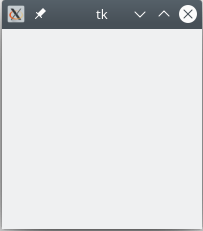
\includegraphics[width=.3\linewidth]{./gfx/12-tk-mini}
\end{tcolorbox}
\end{tcbraster}
%
\begin{itemize}
\item Line 1: Load Module
\item Line 2: Create (Main) Widget
\item Line 3: Set the window's title (as a stand in for fixing the properties)
\item Line 4: Pass Control to tkinter
\end{itemize}
%
\end{frame}

% =========================================================================== %

\begin{frame}{Logic and Structure}
%
\begin{itemize}
\item Object oriented approach (widget \texttt{top})
\item Default Values
	\begin{itemize}
	\item Window Size, title text, position, ...
	\item[\Thus] Methods or ways to change properties
	\end{itemize}
\item Widgets usually are \emph{within} each other widgets (button in window)
	\begin{itemize}
	\item[\Thus] Hierarchical Principle
	\item[\Thus] Children die with their parents
	\end{itemize}
\item Mainloop takes over control
	\begin{itemize}
	\item[\Thus] All definitions need to be done before call to \texttt{mainloop}
	\end{itemize}
\item Widgets need to be interactive
	\begin{itemize}
	\item[\Thus] \emph{Callback functions}: own functions called by \texttt{mainloop}
	\item[\Thus] TkInter handles events, we define the consequences.
	\end{itemize}
\end{itemize}
%
\end{frame}

% =========================================================================== %

\begin{frame}[fragile]
%
\begin{tcbraster}[raster columns=2,
                  raster equal height,
                  nobeforeafter,
                  raster column skip=0.5cm]
\begin{codebox}[Example: Hello World]
\begin{minted}[fontsize=\scriptsize, linenos]{python3}
import tkinter as tk
import tkinter.messagebox as tkmsg

top = tk.Tk()
top.geometry("200x100")

def callback_hello_world():
    tkmsg.showinfo(
        "Hello Python",  # window title
        "Hello World"    # window text
    )

button = tk.Button(
    top,
    text = "Hello",
    command = callback_hello_world
)
button.place(x = 50, y = 50)

top.mainloop()
\end{minted}
\end{codebox}
%
\begin{tcolorbox}[title=Output: Hello World]
\begin{center}
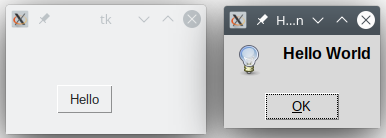
\includegraphics[width=\linewidth]{./gfx/12-tk-button}
\end{center}
\footnotesize
State after clicking the button with label \emph{Hello}.

\vspace{3pt}
Note that the submodule \texttt{tkinter.messagebox} is \emph{not} automatically \inPy{import}ed with tkinter
\end{tcolorbox}
\end{tcbraster}
%
\end{frame}

% =========================================================================== %

\begin{frame}[fragile]{Analysis}
%
\begin{itemize}
\item Define main window
	\begin{itemize}
	\item Change shape: \inPy{top.geometry("200x100")}
		\begin{itemize}
		\item Method \texttt{geometry} takes string argument giving size (and window position)
		\item \inPy{"[width]x[height]+[distance from top]+[distance from left]"}
		\item last two elements may be omitted, or \emph{both} must be present
		\end{itemize}
	\end{itemize}
\item Define button
	\begin{itemize}
	\item Constructor \texttt{tk.Button} with behavior defining arguments
		\begin{itemize}
		\item First Argument: Parent widget
		\item Subsequent arguments: widget-specific keyword arguments
		\end{itemize}
	\item Callback function
		\begin{itemize}
		\item Code to be executed when widget is triggered
		\item Signature (expected arguments, return value) depend on widget \\
			(usually no arguments and return \inPy{None})
		\item Prepare to look up definitions a lot (\zB online)
		\end{itemize}
	\end{itemize}
\item For optional arguments: see link: {\scriptsize \url{https://www.tutorialspoint.com/python3/tk_button.htm}}
\end{itemize}
%
\end{frame}

% =========================================================================== %

\begin{frame}[fragile]{Other Ways of Aranging Widgets}
%
\begin{itemize}
\item Frames
	\begin{itemize}
	\item Widgets, invisible Boxes
	\item Other widgets can be children of frames
	\item Groups for automatic arrangement
	\end{itemize}
\item Method \texttt{pack} of all widgets
	\begin{itemize}
	\item Adds packed widget to frame and (re-)positions all widgets in same frame
	\item Possibly resizes other widgets
	\item Aims for equal space for everything
	\item Optional Parameters
		\begin{itemize}
		\item \inPy{expand=True} -- make packed widget(s) occupy maximum space
		\item \inPy{fill=None} -- refinement of \texttt{expand} option: \\
			expand only in width (\texttt{tk.X}), height (\texttt{tk.Y}) or \texttt{tk.BOTH}
		\item \inPy{side=tk.TOP} -- from where to \enquote{push in} the new widget.\\
			 Alternatives: \texttt{tk.BOTTOM}, \texttt{tk.LEFT}, \texttt{tk.RIGHT}
		\end{itemize}
	\end{itemize}
\item See Link: {\scriptsize \url{https://www.tutorialspoint.com/python3/tk_pack.htm}}
\end{itemize}
%
\end{frame}

% =========================================================================== %

\begin{frame}[fragile]
%
\begin{minipage}{.49\linewidth}
\begin{codebox}[Example: Buttons and Frames...]
\begin{minted}[fontsize=\scriptsize, linenos]{python3}
import tkinter as tk

root = tk.Tk()
root.title("tkinter frames")

frame_top = tk.Frame(root)
frame_top.pack()

frame_bottom = tk.Frame(root)
frame_bottom.pack(side = tk.BOTTOM,
                  fill = tk.X)

button_red = tk.Button(frame_top,
                       text = "Red",
                       fg = "red")
button_red.pack(side = tk.LEFT)

button_green = tk.Button(frame_top,
                         text = "Green",
                         fg = "green")
button_green.pack(side = tk.LEFT)
\end{minted}
\end{codebox}
\end{minipage}
%
\begin{minipage}{.49\linewidth}
\begin{codebox}[... Continued]
\begin{minted}[fontsize=\scriptsize, linenos, firstnumber=last]{python3}
button_blue = tk.Button(frame_top,
                        text = "Blue",
                        fg = "blue")
button_blue.pack(side = tk.LEFT)

button_black = tk.Button(frame_bottom,
                         text = "Black",
                         fg = "black")
button_black.pack(side = tk.BOTTOM,
                  fill = tk.X)

root.mainloop()
\end{minted}
\end{codebox}
\begin{tcolorbox}[title=Output: Buttons and Frames]
\begin{center}
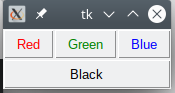
\includegraphics[width=.49\linewidth]{./gfx/12-tk-buttonsframe}
\end{center}
\end{tcolorbox}
\end{minipage}
%
\end{frame}

% =========================================================================== %

\begin{frame}{Tangent: Constants in Modules}
%
\begin{itemize}
\item Observation: \texttt{tk.TOP} et al are actually only strings, holding \inPy{"top"}, etc ...
\item Why use a symbol for this? With the module prefix, it's even more verbose!
\item Maintainability!
	\begin{itemize}
	 \item IDEs keep track of symbols, allow easily renaming them
	 \item ODR (\emph{one definition rule}) -- makes change of the \emph{value} trivial
	 \item More specific than a search and replace (there may be other occurrences of the string \inPy{"top"})
	 \item (Also: some memory saved, as only one pointer is used for each mention of the symbol)
	 \end{itemize} 
\item Common practice across most languages
	\begin{itemize}
	\item C-like languages use \mintinline{c}{enum}s for this
	\item C++: \mintinline{c}{enum class} for better type safety (\zB automatically defines namespace)
	\item Python has a module \texttt{enum} which offers some neat features
	\end{itemize}
\end{itemize}
%
\end{frame}

% =========================================================================== %

\begin{frame}[fragile]{Tangent: Accessing Tangent Properties Post Construction}
%
\begin{itemize}
\item Attributes like widget text can be accessed (read/write) after the widget has been constructed
\item Just treat them like a \inPy{dict}; keys are the same as for the CTor
\item Examples
	\begin{itemize}
	\item Read access: \inPy{caption = some_button["text"]}
	\item Write access: \inPy{some_button["state"] = tk.DISABLED} (counterpart. \texttt{tk.NORMAL})
	\end{itemize}
\item Alternative, if you want to update several attributes at once: \inPy{widget.configure(dict_of_attributes)}
\item Read all the attributes at once: \inPy{dict_of_attributes = widget.configure()}
\end{itemize}
%
\end{frame}

% =========================================================================== %

\begin{frame}[fragile]{Other Ways of Aranging Widgets}
%
\begin{columns}[T]
\column{.5\linewidth}
\begin{itemize}
\item Method \texttt{grid}
	\begin{itemize}
	\item Arrange widgets on a grid
	\item Optional arguments \texttt{row} and \texttt{col} -- integers defining position
	\item Grid is automatically resized for each added element
	\item More optional parameters: {\scriptsize \url{https://www.tutorialspoint.com/python3/tk_grid.htm}}
	\end{itemize}
\end{itemize}
\begin{center}
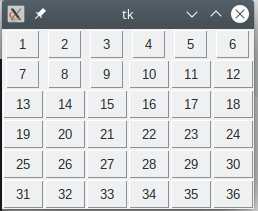
\includegraphics[width=.35\linewidth]{./gfx/12-tk-grid}
\end{center}
%
\column{.5\linewidth}
\begin{codebox}[Example: \texttt{grid}]
\begin{minted}[fontsize=\scriptsize, linenos]{python3}
import tkinter as tk
root = tk.Tk()

number = 1
for row in range(6):
    for column in range(6):
        tk.Button(root,
                  text=str(number),
                  borderwidth=1
        ).grid(row=row,
               column=column
        )
        number += 1

root.mainloop()
\end{minted}
\end{codebox}
\end{columns}
%
\end{frame}

% =========================================================================== %

\begin{frame}[fragile]{Tangent: Parametrized Callbacks}
%
\begin{itemize}
\item Conceivable: want callbacks; same for all buttons, depending on button ID
	\begin{itemize}
	\item E.\;g.: \inPy{print(f"Clicked Button {i}")}
	\end{itemize}
\item But: callback must not take argument and \texttt{number} is overwritten 
	\begin{itemize}
	\item[\Thus] \inPy{print(f"Clicked Button {number}")} would print same value for all buttons
	\item[\Thus] Need to persist current value somewhere
	\end{itemize}
\item Solution 1 (explicit): own function for each button
	\begin{itemize}
	\item Bad because not DRY\footnote{\emph{Don't Repeat Yourself}}
	\end{itemize}
\item Solution 2 (clean but still verbose): callable class
	\begin{itemize}
	\item Instance attribute \texttt{buttonID} and method \inPy{__call__}
	\item Good idea for more sophisticated mechanisms, overkill for \enquote{simply print the ID}
	\end{itemize}
\item Solution 3 (hack): hide it in default argument of instance of a \inPy{lambda}
	\begin{itemize}
	\item \inPy{command = lambda i=number: print(f"Clicked Button {i}")}
	\end{itemize}
\end{itemize}
%
\end{frame}

% =========================================================================== %

\begin{frame}[fragile]{Widgets with States -- Variable-Mechanism}
%
\vspace{-6pt}
\begin{columns}[T]
\column{.7\linewidth}
\begin{itemize}
\item Widgets like checkboxes, radiobuttons, ...: state
	\begin{itemize}
	\item checked/unchecked, option x/y, ...
	\end{itemize}
\item Access via external variable 
	\begin{itemize}
	\item External to the widget \Thus No \inPy{widget.get_checked()}
	\end{itemize}
\item Instead: register \enquote{callback-variable}
	\begin{itemize}
	\item Optional CTor argument \texttt{variable = ...}
	\item Variable is changed when the widget is used
	\item Value depends on kind and setup of widget
	\end{itemize}
\item Variable is an instance of one of several Tk-classes
	\begin{itemize}
	\item \texttt{tk.IntVar} -- stores an \inPy{int} \\
		(\thus checkboxes and radiobuttons)
	\item \texttt{tk.StringVar} -- stores \inPy{str}ings
	\item Updates to these variables will directly affect linked controls
	\item (This is why extra classes are needed)
	\end{itemize}
\end{itemize}
%
\column{.2\linewidth}
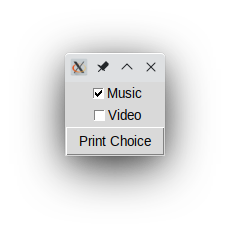
\includegraphics[width=\linewidth]{./gfx/12-tk-checkboxes}

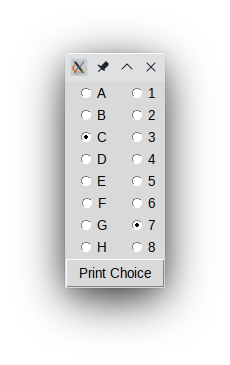
\includegraphics[width=\linewidth]{./gfx/12-tk-radiobuttons}
\end{columns}
%
\end{frame}

% =========================================================================== %

\begin{frame}[fragile]
%
\begin{tcbraster}[raster columns=2,
                  raster equal height,
                  nobeforeafter,
                  raster column skip=0.5cm]
\begin{codebox}[Example: Two Checkboxes ...]
\begin{minted}[fontsize=\scriptsize, linenos]{python3}
import tkinter as tk

top = tk.Tk()

checkbox_var_1 = tk.IntVar()
checkbox_var_2 = tk.IntVar()

def choice_text():
    if checkbox_var_1.get() == 1 and \
       checkbox_var_2.get() == 1:
        result = "Music and Video"
    elif checkbox_var_1.get() == 1:
        result = "Music only"
    elif checkbox_var_2.get() == 1:
        result = "Video only"
    else:
        result = "Nothing"
    return result
\end{minted}
\end{codebox}
%
\begin{codebox}[... Continued]
\begin{minted}[fontsize=\scriptsize, linenos, firstnumber=last]{python3}
checkbox_1 = tk.Checkbutton(
    top, 
    text="Music",
    variable=checkbox_var_1)
checkbox_1.pack()

checkbox_2 = tk.Checkbutton(
    top,
    text="Video",
    variable=checkbox_var_2)
checkbox_2.pack()

button = tk.Button(
    top,
    text="Print Choice",
    command=lambda:print(choice_text()))
button.pack()

top.mainloop()
\end{minted}
\end{codebox}
\end{tcbraster}
%
\end{frame}

% =========================================================================== %

\begin{frame}[fragile]
%
\begin{tcbraster}[raster columns=2,
                  raster equal height,
                  nobeforeafter,
                  raster column skip=0.5cm]
\begin{codebox}[Example: Radiobuttons ...]
\begin{minted}[fontsize=\scriptsize, linenos]{python3}
import tkinter as tk

top = tk.Tk()
rows = 5

optionL = tk.IntVar()
optionR = tk.IntVar()

def getChoiceText():
    return chr(optionL.get() + 65) + \
           str(optionR.get())

for i in range(rows) :
    tk.Radiobutton(
        text=chr(i + 65),
        variable=optionL,
        val=i
    ).grid(
        row=i, column=0
    )
\end{minted}
\end{codebox}
%
\begin{codebox}[... Continued]
\begin{minted}[fontsize=\scriptsize, linenos, firstnumber=last]{python3}
for i in range(rows) :
    tk.Radiobutton(
        text=str(i),
        variable=optionR,
        val=i
    ).grid(
        row=i, column=1
    )

tk.Button(
    text="Print Choice",
    command = lambda :
        print( getChoiceText() )
).grid(
    row=rows, column=0,
    columnspan=2
)

top.mainloop()
\end{minted}
\end{codebox}
\end{tcbraster}
%
\end{frame}

% =========================================================================== %

\begin{frame}[fragile]{Textboxes}
%
%
\begin{itemize}
\item Class \texttt{tk.Entry} -- one line textbox
	\begin{itemize}
	\item \emph{Compatible} with \texttt{variable} mechanism
	\item Would then take an \texttt{tk.StringVar}
	\item Not strictly necessary (but sometimes convenient)
	\item Callback \texttt{command} called each time the state changes (each keypress)
	\item String \texttt{show} -- hide typed characters (for passwords)
	\item See link: {\scriptsize \url{https://www.tutorialspoint.com/python3/tk_entry.htm}}
	\end{itemize}
\item Class \texttt{tk.Text} -- multiline textbox
	\begin{itemize}
	\item Similar attributes
	\item No \texttt{show} feature
	\item Rich Text Capacity -- \zB coloured text
	\item See link: {\scriptsize \url{https://www.tutorialspoint.com/python3/tk_text.htm}}
	\end{itemize}
\item Class \texttt{tk.Label} -- Static Text Display
	\begin{itemize}
	\item Oten used to hint what user should input here
	\item Can also show images
	\end{itemize}
\end{itemize}
%
\end{frame}

% =========================================================================== %

\begin{frame}[fragile]
%
\begin{tcbraster}[raster columns=2,
                  raster equal height,
                  nobeforeafter,
                  raster column skip=0.5cm]
\begin{codebox}[Example: Entries...]
\begin{minted}[fontsize=\scriptsize, linenos]{python3}
import tkinter as tk

top = tk.Tk()

frame_top = tk.Frame(top)
frame_top.pack(side=tk.TOP)

frame_btm = tk.Frame(top)
frame_btm.pack(side=tk.BOTTOM,
               fill=tk.X)

label = tk.Label(frame_top,
                 text = "User Name"
)
label.pack(side = tk.LEFT)
\end{minted}
\end{codebox}
%
\begin{codebox}[... Continued]
\begin{minted}[fontsize=\scriptsize, linenos, firstnumber=last]{python3}
entry = tk.Entry(frame_top)
entry.pack(side = tk.RIGHT)

button = tk.Button(
    frame_btm,
    text="show",
    command = lambda: print(entry.get())
)
button.pack(fill=tk.X)

top.mainloop()
\end{minted}
\end{codebox}
\end{tcbraster}
%
%\begin{tcolorbox}[title=Output: Buttons and Frames]
\begin{center}
	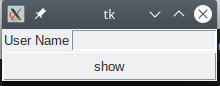
\includegraphics[width=.25\linewidth]{./gfx/12-tk-entry}
\end{center}
%\end{tcolorbox}
%
\end{frame}

% =========================================================================== %

\begin{frame}[fragile]{Listboxes}
%
\begin{itemize}
\item Select one or multiple strings out of a list
\item Widget \texttt{tk.Listbox}
	\begin{itemize}
	\item Important Attributes to the Constructor
		\begin{itemize}
		\item \texttt{height} -- number of lines
		\item \texttt{selectmode} -- \texttt{tk.SINGLE} (select one item), \texttt{tk.MULTIPLE} (select several items) or \texttt{tk.EXTEND} (select adjacent items)
		\item \emph{No} command option
		\end{itemize}
	\item Does have an internal state
		\begin{itemize}
		\item Tracks listed strings and selection
		\end{itemize}
	\item Important Methods 
		\begin{itemize}
		\item \texttt{insert(index, string)} -- adds an option
		\item \texttt{delete(index)} -- removes an option
		\item \texttt{activate(index)} -- select one item
		\item \texttt{curselection()} -- returns \inPy{tuple} of selected lines (or empty \inPy{tuple})
		\item \texttt{get(index)} -- returns string in line \texttt{index}.
		\item \texttt{get(start, stop)} -- returns \inPy{tuple} of items with indices \texttt{start} till \texttt{stop}, \emph{included}
		\end{itemize}
	\end{itemize}
\end{itemize}
%
\end{frame}

% =========================================================================== %

\begin{frame}[fragile]{Example: Listboxes}
%
\begin{columns}[T]
\column{.5\linewidth}
\begin{itemize}
\item Aim: Buttons add predefined lines to Listbox
\item Button \texttt{>} adds user text to listbox
\item Button \texttt{remove} deletes a selected line from listbox
\item Button \texttt{order} displays listbox content and terminates the program
\end{itemize}
%
\column{.5\linewidth}
\begin{tcolorbox}[title=Pizza Order Tool]
\begin{center}
	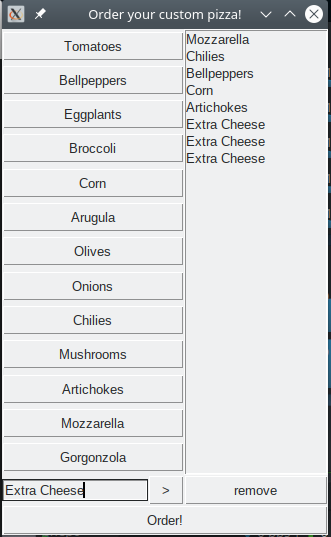
\includegraphics[width=.5\linewidth]{./gfx/12-tk-listbox}
\end{center}
\end{tcolorbox}
\end{columns}
%
\end{frame}

% =========================================================================== %

\begin{frame}[fragile]
%
\begin{codebox}[Example: Pizza Order Tool (1)]
\begin{minted}[linenos, fontsize=\scriptsize]{python3}
import tkinter as tk
import tkinter.messagebox as msg

defaultOptions = ("Tomatoes", "Bellpeppers", "Eggplants", "Broccoli", "Corn",
                  "Arugula", "Olives", "Onions", "Chilies", "Mushrooms",
                  "Artichokes", "Mozzarella", "Gorgonzola")

# numerical constants: describe width and height of the interface
N = len(defaultOptions)
W = 6

top = tk.Tk()
top.title("Order your custom pizza!")

buttons = []
for i, ingredient in enumerate(defaultOptions) :
    buttons.append(tk.Button(
        top,
        text = ingredient,
        command = lambda c=i: lst.insert(tk.END, buttons[c]["text"])
    ))
\end{minted}
\end{codebox}
%
\end{frame}

% =========================================================================== %

\begin{frame}[fragile]
%
\begin{codebox}[Example: Pizza Order Tool (2)]
\begin{minted}[linenos, fontsize=\scriptsize, firstnumber=last]{python3}
    buttons[i].grid(
        column = 0, row = i,
        columnspan = W,     # use W cells in the grid
        sticky = "WE"       # fill the entire width of the grid
    )

txt = tk.Entry(top)
txt.grid(
    column = 0, row = N,
    columnspan = W - 1
)

tk.Button(
    top,
    text = ">",
    command = lambda : lst.insert(tk.END, txt.get())
).grid(column = W - 1, row = N)

lst = tk.Listbox(top, height = 2*N)
lst.grid(column = W + 1, row = 0, rowspan=N)
\end{minted}
\end{codebox}
%
\end{frame}

% =========================================================================== %

\begin{frame}[fragile]
%
\begin{codebox}[Example: Pizza Order Tool (3)]
\begin{minted}[linenos, fontsize=\scriptsize, firstnumber=last]{python3}
tk.Button(
    top,
    text = "remove",
    command = lambda :
        lst.delete(*lst.curselection()) if len(lst.curselection()) else None
).grid(
    column = W + 1, row = N,
    sticky = "WE"
)

def getOrderText () :
    result = "One pizza with"
    if lst.size() == 0 :
        result += " nothing"
    else :
        for item in lst.get(0, tk.END) :
            result += "\n* " + item
    return result
\end{minted}
\end{codebox}
%
\end{frame}

% =========================================================================== %

\begin{frame}[fragile]
%
\begin{codebox}[Example: Pizza Order Tool (4)]
\begin{minted}[linenos, fontsize=\scriptsize, firstnumber=last]{python3}
def orderMsgBox () :
    msg.showinfo("your Order", getOrderText())
    top.destroy()    # closes the main window

tk.Button(
    top,
    text = "Order!",
    command = orderMsgBox
).grid(
    column = 0, row = N + 1,
    columnspan = W + 2,
    sticky = "WE"
)

top.mainloop()
\end{minted}
\end{codebox}
%
\end{frame}

% =========================================================================== %

\begin{frame}[fragile]{Pre-Built Dialogs}
%
\begin{itemize}
\item Module \texttt{tk.filedialog} -- load file / save file / select directory dialogs
\item Module \texttt{tk.colorchooser} -- get hex colour value from user
\item Module \texttt{tk.messagebox} -- different Symbols and pre-defined buttons
\item All of them: See \url{https://tkdocs.com/tutorial/windows.html#dialogs}
\end{itemize}
%
\begin{hintbox}[Have a look around]
This lecture has, again, only shown you a fraction of what tkinter can do.

Browse the links provided to see which widgets are supported and how they behave. Use your search engine of choice to find example codes on many a scenario.
\end{hintbox}
%
\end{frame}

% =========================================================================== %

\begin{frame}[fragile]{MatPlotLib Integration}
%
\begin{itemize}
\item MatPlotLib provides TkInter integration
\item Draw your plots normally, using the object oriented interface
	\begin{itemize}
	\item \inPy{figure = plt.figure(...)}
	\item \inPy{axs = figure.subplot(...)}
	\item \inPy{axs.plot(...)}
	\item DO NOT \texttt{figure.show()}!
	\end{itemize}
\item Create an interface between MatPlotLib and TkInter
	\begin{itemize}
	\item \inPy{from matplotlib.backends.backend_tkagg import FigureCanvasTkAgg}
	\item \inPy{interface = FigureCanvasTkAgg(figure, master=parent_widget)}
	\item \inPy{interface.get_tk_widget().pack(...)}
	\end{itemize}
\item Updating Plots at runtime
	\begin{itemize}
	\item \inPy{axs.cla()	# clear plot ...}
	\item \inPy{axs.plot(...)	# ... and draw your new content}
	\item \inPy{interface.draw()}
	\end{itemize}
\end{itemize}
%
\end{frame}

% =========================================================================== %